\documentclass[[12pt,twoside]{book}
\usepackage{_my_document_style}
\begin{document}
%
\begin{myExampleX}{Lift gradient of a finite wing. Effect of aspect ratio}{\ding{46}}% \ \Keyboard\ %
\label{example:Lift:Gradient:Aspect:Ratio:Effect}
%
\noindent
We want to calculate the lift gradient \smash{$C_{L_\mathlarger{\alpha}}$}
of a wing similar to that one of the example~\ref{example:Lift:Gradient:Of:A:Finite:Wing}
verifying the effect of the aspect ratio variation.

%-------------------------------------------------
\def\mySpanWingMT{26.800000}
\def\myMach{0.700000}
\def\myAspectRatioWing{7.108753}
\def\myChordRootWingMT{5.200000}
\def\myChordTipWingMT{2.340000}
\def\myTaperRatioWing{0.450000}
\def\myAreaWingMTsquared{101.036000}
\def\myCoeffAChordWing{-0.213433}
\def\myCoeffBChordWingMT{5.200000}
\def\myCLAlphaRootWingRAD{6.150000}
\def\myCLAlphaTipWingRAD{6.050000}
\def\myCoeffAClalphaWingRADMT{-0.007463}
\def\myCoeffAClalphaWingDEGMT{-0.000130}
\def\myCoeffBClalphaWingRAD{6.150000}
\def\myCLAlphaMeanWingRAD{6.106322}
\def\myCLAlphaMeanWingDEG{0.106575}
\def\myInducedDragFactorWing{0.900000}
\def\myCLAlphaWingRAD{4.683465}
\def\myCLAlphaWingDEG{0.081742}

\let\mySpanWingAMT\mySpanWingMT
\let\myAreaWingAMTsquared\myAreaWingMTsquared
\let\myAspectRatioWingA\myAspectRatioWing
\let\myCLAlphaMeanWingARAD\myCLAlphaMeanWingRAD
\let\myCLAlphaMeanWingADEG\myCLAlphaMeanWingDEG
\let\myCLAlphaWingARAD\myCLAlphaWingRAD
\let\myCLAlphaWingADEG\myCLAlphaWingDEG
%-------------------------------------------------
For this wing we have:

\smallskip
\noindent
\adjustbox{center=\textwidth}{%
$b=\SI[round-precision=2]{\mySpanWingAMT}{\meter}$,
$\AR=\SI[round-precision=2]{\myAspectRatioWingA}{}$,
$S=\SI[round-precision=2]{\myAreaWingAMTsquared}{\metre^2}$,
\smash{$\bar{C}_{\ell_\mathlarger{\alpha}}=\SI[round-precision=3]{\myCLAlphaMeanWingRAD}{\radian^{-1}}$}
}

\smallskip
\noindent
\adjustbox{center=\textwidth}{%
$C_{L_\mathlarger{\alpha}}
  =\mathunderline{mydarkblue}{ \SI[round-precision=2]{\myCLAlphaWingARAD}{\radian^{-1}} }
  =\mathunderline{mydarkblue}{ \SI[round-precision=3]{\myCLAlphaWingADEG}{\deg^{-1}} }
$
}

\smallskip
%-------------------------------------------------
\def\mySpanWingMT{21.440000}
\def\myMach{0.700000}
\def\myAspectRatioWing{5.687003}
\def\myChordRootWingMT{5.200000}
\def\myChordTipWingMT{2.340000}
\def\myTaperRatioWing{0.450000}
\def\myAreaWingMTsquared{80.828800}
\def\myCoeffAChordWing{-0.266791}
\def\myCoeffBChordWingMT{5.200000}
\def\myCLAlphaRootWingRAD{6.150000}
\def\myCLAlphaTipWingRAD{6.050000}
\def\myCoeffAClalphaWingRADMT{-0.009328}
\def\myCoeffAClalphaWingDEGMT{-0.000163}
\def\myCoeffBClalphaWingRAD{6.150000}
\def\mySweepQuarterChordWingDEG{0.000000}
\def\mySweepQuarterChordWingRAD{0.000000}
\def\myCLAlphaMeanWingRAD{6.106322}
\def\myCLAlphaMeanWingDEG{0.106575}
\def\myInducedDragFactorWing{0.900000}
\def\myCLAlphaWingRAD{4.425656}
\def\myCLAlphaWingDEG{0.077242}

\let\mySpanWingBMT\mySpanWingMT
\let\myAreaWingBMTsquared\myAreaWingMTsquared
\let\myAspectRatioWingB\myAspectRatioWing
\let\myCLAlphaMeanWingBRAD\myCLAlphaMeanWingRAD
\let\myCLAlphaMeanWingBDEG\myCLAlphaMeanWingDEG
\let\myCLAlphaWingBRAD\myCLAlphaWingRAD
\let\myCLAlphaWingBDEG\myCLAlphaWingDEG
%-------------------------------------------------
For a wing of equal root chord and taper ratio, but of wingspan $b'$ decreased by $20\%$ compared to $b$ we have:

\smallskip
\noindent
\adjustbox{center=\textwidth}{%
$b'=\SI[round-precision=2]{\mySpanWingBMT}{\meter}$,
$\AR'=\SI[round-precision=2]{\myAspectRatioWingB}{}$,
$S'=\SI[round-precision=2]{\myAreaWingBMTsquared}{\metre^2}$,
\smash{$\bar{C}_{\ell_\mathlarger{\alpha}}'=\SI[round-precision=4]{\myCLAlphaMeanWingRAD}{\radian^{-1}}$}
}

\smallskip
\noindent
\adjustbox{center=\textwidth}{%
$C_{L_\mathlarger{\alpha}}'
  =\mathunderline{mydarkblue}{ \SI[round-precision=2]{\myCLAlphaWingBRAD}{\radian^{-1}} }
  =\mathunderline{mydarkblue}{ \SI[round-precision=3]{\myCLAlphaWingBDEG}{\deg^{-1}} }
$
}

\smallskip
%-------------------------------------------------
\def\mySpanWingMT{32.160000}
\def\myMach{0.700000}
\def\myAspectRatioWing{8.530504}
\def\myChordRootWingMT{5.200000}
\def\myChordTipWingMT{2.340000}
\def\myTaperRatioWing{0.450000}
\def\myAreaWingMTsquared{121.243200}
\def\myCoeffAChordWing{-0.177861}
\def\myCoeffBChordWingMT{5.200000}
\def\myCLAlphaRootWingRAD{6.150000}
\def\myCLAlphaTipWingRAD{6.050000}
\def\myCoeffAClalphaWingRADMT{-0.006219}
\def\myCoeffAClalphaWingDEGMT{-0.000109}
\def\myCoeffBClalphaWingRAD{6.150000}
\def\mySweepQuarterChordWingDEG{0.000000}
\def\mySweepQuarterChordWingRAD{0.000000}
\def\myCLAlphaMeanWingRAD{6.106322}
\def\myCLAlphaMeanWingDEG{0.106575}
\def\myInducedDragFactorWing{0.900000}
\def\myCLAlphaWingRAD{4.872699}
\def\myCLAlphaWingDEG{0.085045}

\let\mySpanWingCMT\mySpanWingMT
\let\myAreaWingCMTsquared\myAreaWingMTsquared
\let\myAspectRatioWingC\myAspectRatioWing
\let\myCLAlphaMeanWingCRAD\myCLAlphaMeanWingRAD
\let\myCLAlphaMeanWingCDEG\myCLAlphaMeanWingDEG
\let\myCLAlphaWingCRAD\myCLAlphaWingRAD
\let\myCLAlphaWingCDEG\myCLAlphaWingDEG
%-------------------------------------------------
Similarly, for a wingspan $b''$ increased by $20\%$ compared to $b$ we have:

\smallskip
\noindent
\adjustbox{center=\textwidth}{%
$b''=\SI[round-precision=2]{\mySpanWingCMT}{\meter}$,
$\AR''=\SI[round-precision=2]{\myAspectRatioWingC}{}$,
$S''=\SI[round-precision=2]{\myAreaWingCMTsquared}{\metre^2}$,
\smash{$\bar{C}_{\ell_\mathlarger{\alpha}}''=\SI[round-precision=4]{\myCLAlphaMeanWingRAD}{\radian^{-1}}$}
}

\smallskip
\noindent
\adjustbox{center=\textwidth}{%
$C_{L_\mathlarger{\alpha}}''
  =\mathunderline{mydarkblue}{ \SI[round-precision=2]{\myCLAlphaWingCRAD}{\radian^{-1}} }
  =\mathunderline{mydarkblue}{ \SI[round-precision=3]{\myCLAlphaWingCDEG}{\deg^{-1}} }
$
}

\medskip
Lift gradient values $C_{L_\mathlarger{\alpha}}'$ and $C_{L_\mathlarger{\alpha}}''$
are calculated applying the procedure of the example~\ref{example:Lift:Gradient:Of:A:Finite:Wing}.
It is observed that for a gradually increasing aspect ratio
($\AR' < \AR < \AR''$) the gradient of the lifting line of the wing increases
($C_{L_\mathlarger{\alpha}}' < C_{L_\mathlarger{\alpha}} < C_{L_\mathlarger{\alpha}}''$).

See the figure~\ref{fig:CLAlpha:Wing:Planforms:B} for a graphic confirmation of previous results.
\end{myExampleX}
\begin{figure}
  [t]%[H]%[!htbp]
  %\centering
  %\checkoddpage
  %\centering
    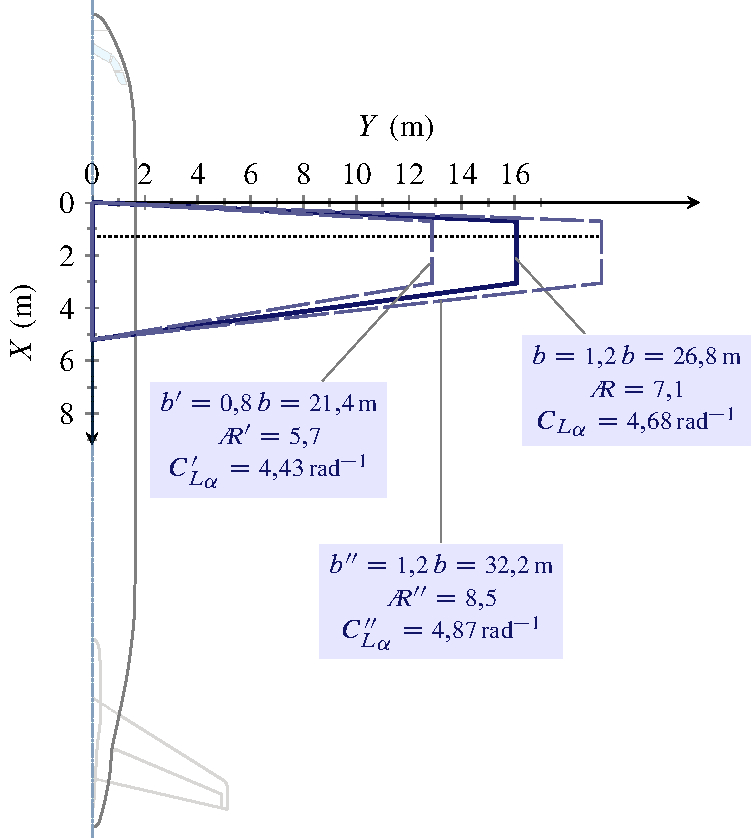
\includegraphics[width=0.70\textwidth]{Chapter_2/lift_gradient_aspect_ratio_effect/wing_planforms_drawing.pdf}
  \caption{\finalhyphendemerits=1000
           Planform with different wingspans but with the same root and tip chords.}
  \label{fig:CLAlpha:Wing:Planforms:B}%
\end{figure}
\end{document}